\documentclass[a4paper,titlepage]{article}
\title{CT Projekt: Raycasting engine (Hundefels 2D)}
\author{Christian Korn}
\date{20.10.2021 - 11.01.2022}

\usepackage[ngerman]{babel}
\usepackage{graphicx}
\usepackage{amssymb}

\begin{document}
\maketitle
\tableofcontents

\newpage

\section{Ziele}

\subsection{Muss-Ziele}
Wenn diese Ziele nicht erreicht werden, wird das Projekt als Fehlschlag angesehen.

\begin{itemize}
\item Anzeigen eines 2D Levels in 2,5D (Raycasting Methode) \checkmark
\item Bewegungsfreiheit im Level (Translation und Rotation) \checkmark
\end{itemize}

\subsection{Soll-Ziele}
Diese Ziele müssen nicht unbedingt erreicht werden, sind aber für einen vollen Erfolg nötig.

\begin{itemize}
\item Laden von Leveln aus Dateien \checkmark
\item Anzeigen von anderen Objekten im Level (z.B. Gegner, Items) \checkmark
\item Kollisionserkennung \checkmark
\end{itemize}

\subsection{Kann-Ziele}
Diese Ziele sind nicht nötig, können aber nach Vollendung der Höheren Ziele in Angriff genommen werden.

\begin{itemize}
\item Gegner KI
\item Schießen
\item Sprites
\item Texturen für Wände
\item visuelle Effekte (view bobbing, Blutspritzer)
\end{itemize}

\newpage

\section{Verwendete Technologien}

\subsection{Python}

Das Projekt wurde mit Python \verb|3.9.7| erstellt, müsste aber auch in späteren Versionen funktionieren.

\subsubsection*{Externe Libraries}

\begin{itemize}
	\item Pygame: Installation mit ``\verb|pip install pygame|''
	Verwendet für Darstellung.
	\item Numba: Installation mit ``\verb|pip install numba|''
	Für `magische' Leistungsverbesserungen von besonders aufwändigen Funktionen durch JIT-Compilierung.
\end{itemize}

\subsubsection*{IDE}

Es wurde die PyCharm Community Edition verwendet.

\subsection{Dokumentation}

Die Projektdokumentation wurde mit \LaTeX erstellt,
UML Klassendiagramme wurden mit YUML erstellt.

\subsection{Versionskontrollsystem}

Das GIT Repository kann unter \verb|https://github.com/MacAphon/hundefels2d| gefunden werden.

\newpage
\section{Mathematische Funktionsweise}

Die Berechnungen werden 1 mal pro Frame ausgeführt. Idealerweise heißt das, dass sie 60 mal pro Sekunde erfolgen. wenn die Rechenleistung nicht ausreicht wird eine Warnung angezeigt.

\subsection{Bewegung}

Der aktuelle Bewegungszustand und die Position werden in den Variablen \verb|_state|, \verb|_movement| und \verb|_position| gespeichert.

\verb|_state| enthält die x- und y-Bewegungsgeschwindigkeit, sowie Rotationsgeschwindigkeit relativ zum Spieler, \verb|_movement| enthält die absoluten Geschwindikeitswerte.\\

Für jeden Frame wird überprüft, welche tasten aktuell gedrückt sind und dementsprechend \verb|_state| angepasst.

Aus \verb|_state| wird dann \verb|_movement| berechnet und diese Werte mit \verb|_position| addiert.

\subsection{Darstellung}

\subsubsection*{Welt}

Vom Spieler ausgehend werden Strahlen in Paaren ausgesendet:

Der horizontale Strahl überprüft bei vertikalen Linien, der vertikale Strahl bei horizontalen Linien.
Mit dem Unterschied der Richtung funktionieren beide insgesamt gleich, die Erklärung konzentriert sich daher auf den horizontalen Strahl.\\

Zuerst wird der x-Wert des Strahls $x_{ray}$ auf die nächste Linie gesetzt, danach der y-Wert $y_{ray}$ mit folgender Formel bestimmt: 

$$y_{ray} = x_{player}-x_{ray}*\frac{-1}{\tan(\alpha_{ray})}+y_{player}$$

Nun wird der Strahl wiederholt um 1 in $x$-Richtung und um

$$-block\_size * \frac{-1}{\tan(\alpha_{ray}}$$

in $y$-Richtung verschoben. Nach jedem Verschieben wird überprüft, um es sich beim neuen Block um eine Wand handelt, wenn ja wird abgebrochen und die zurückgelegte Entfernung, sowie die x- und y-Koordinaten des Strahls zurückgegeben.\\

Von den zwei so berechneten Werten wird nun der kürzere Strahl ausgewählt, auf der Karte gezeichnet und als vertikale Linie  der Länge

$$v\_offset = \frac{1}{dist + 0,001} * 9000 $$

im Viewport angezeigt ($dist$ ist die Länge des Strahls, die zwei festen Werte verhindern, dass durch 0 geteilt wird und erhöhen den Wert auf eine sichtbare Länge).

\newpage

\subsubsection*{Beispiel}
\setlength{\unitlength}{1cm}
Horizontaler Check, vertikaler Strahl:\\\\
\begin{picture}(5,4)
	% Gitternetz
	\multiput(0,0)(1,0){6}{\line(0,1){4}}
	\linethickness{0.4mm}
	\multiput(0,0)(0,1){5}{\line(1,0){5}}
	\thinlines
	% Wand
	\multiput(0,0)(0.1,0){50}{\line(0,1){1}}
	% Spieler und Sichtlinie
	\put(1,3){\circle*{0.3}}
	\thicklines
	\put(1,3){\vector(4,-3){2.7}}
	% Kreuzpunkte
	\linethickness{0.6mm}
	\put(2.35,1.75){\line(0,1){0.5}}
	\put(2.1,2){\line(1,0){0.5}}
	\put(3.68,0.75){\line(0,1){0.5}}
	\put(3.43,1){\line(1,0){0.5}}
\end{picture}\\\\
Vertikaler Check, horizontaler Strahl:\\\\
\begin{picture}(5,4)
	% Gitternetz
	\linethickness{0.4mm}
	\multiput(0,0)(1,0){6}{\line(0,1){4}}
	\thinlines
	\multiput(0,0)(0,1){5}{\line(1,0){5}}
	% Wand
	\multiput(0,0)(0.1,0){50}{\line(0,1){1}}
	% Spieler und Sichtlinie
	\put(1,3){\circle*{0.3}}
	\thicklines
	\put(1,3){\vector(4,-3){3}}
	% Kreuzpunkte
	\linethickness{0.6mm}
	\put(2,2){\line(0,1){0.5}}
	\put(1.75,2.25){\line(1,0){0.5}}
	\put(3,1.25){\line(0,1){0.5}}
	\put(2.75,1.5){\line(1,0){0.5}}
	\put(4,0.5){\line(0,1){0.5}}
	\put(3.75,0.75){\line(1,0){0.5}}
\end{picture}

\subsubsection*{Entities}

Die Formel für die Berechnung der x-Position einer Entity im Viewport wird mit folgender Formel berechnet:

$$
x_{Fenster} = \frac{tan^{-1}{\frac{\Delta y_{entity, player}}{\Delta x_{entity, player}}} + \alpha_{player} + \beta_{player}}{\beta_{player}}*Fensterbreite
$$


$\alpha_{player}$ ist die Blickrichtung des Spielers, $\beta_{player}$ das Blickfeld.

Einige Korrekturen werden dabei noch vorgenommen, um die Position der Entity auf dem Bildschirm nicht umherspringen zu lassen.\\

Zuerst werden die Strahlen hinter der Entity angezeigt, dann die Entity selbst und zuletzt die Strahlen vor der Entity.

\newpage

\section{Programmaufbau}

Die UML-Diagramme können in voller Größe im Git-Repo in \verb|dokumentation/img| gefunden werden. Die relevanten Dateien sind \verb|yuml-1.png|, \verb|yuml-2.png|, \verb|yuml-3.png|, \verb|yuml-4.png| und \verb|yuml-final.png|.
 
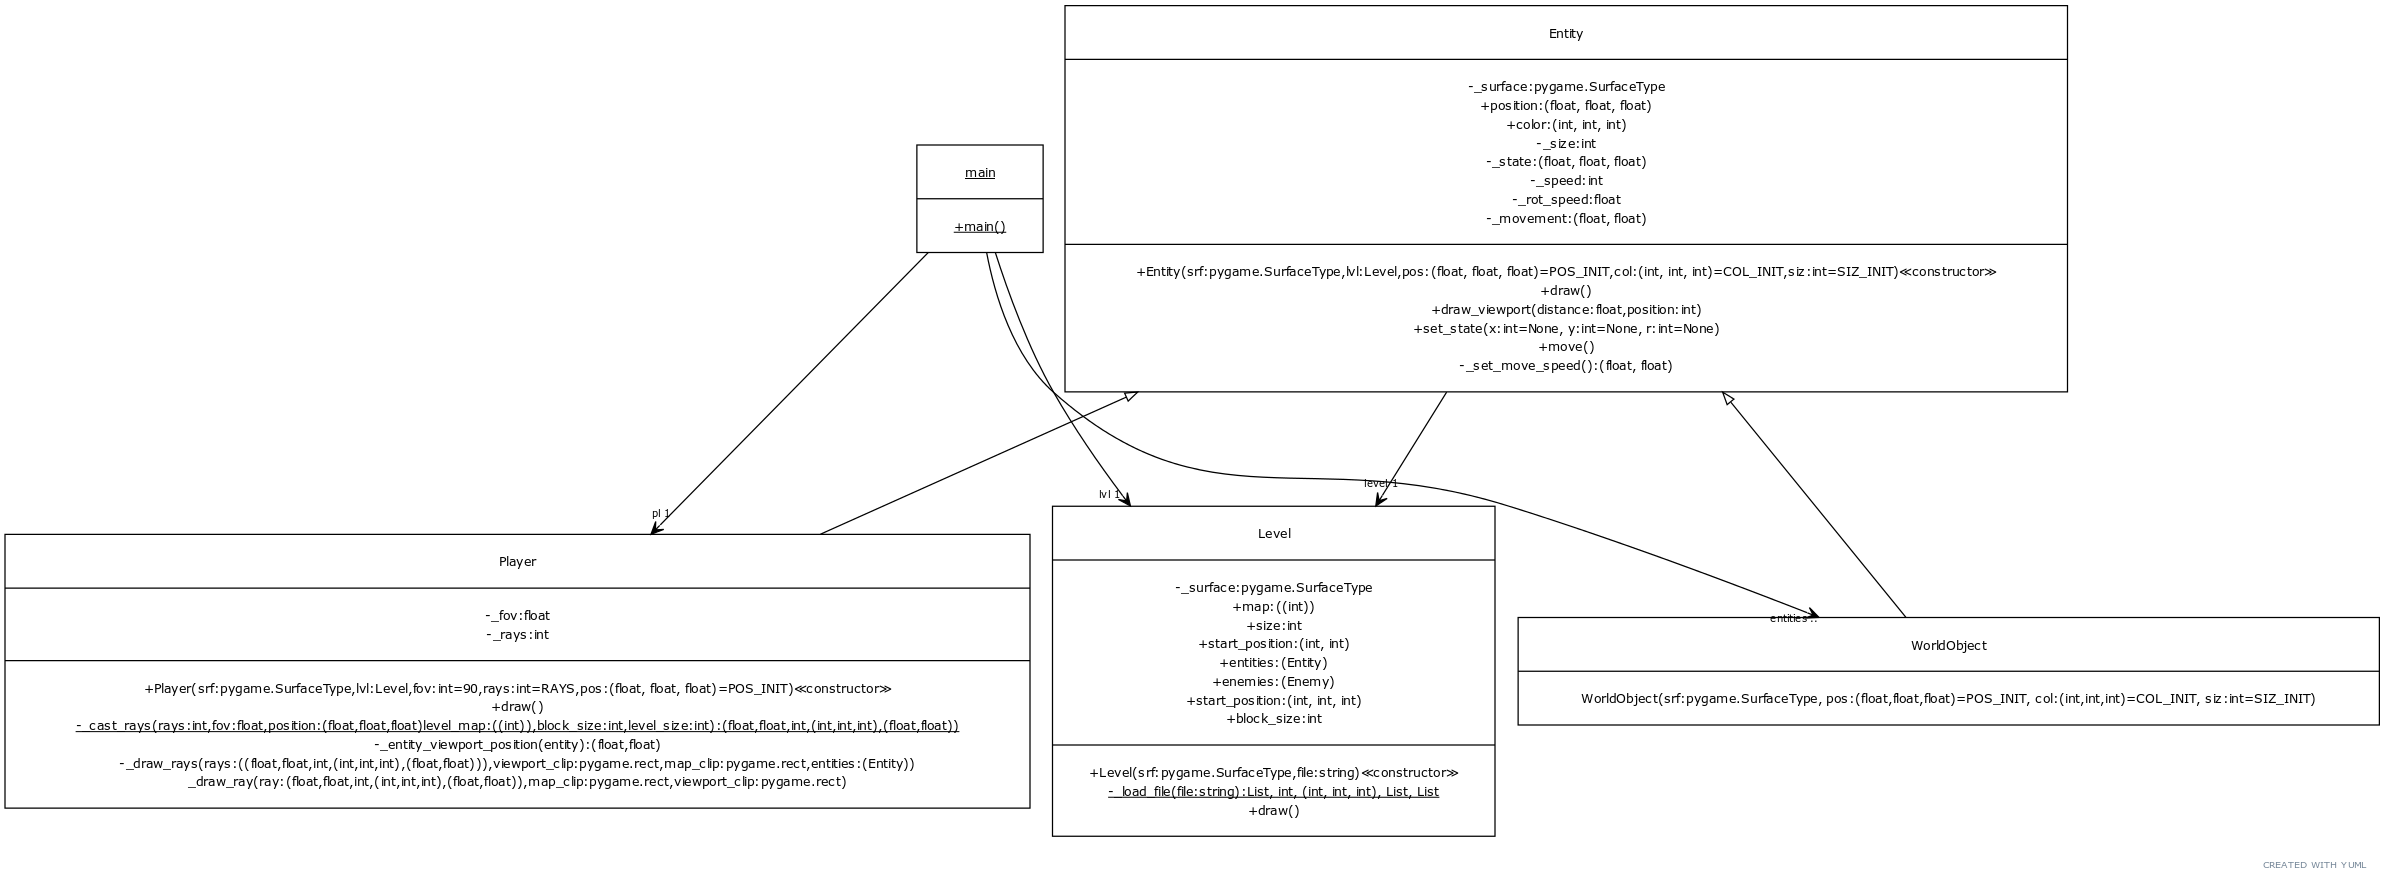
\includegraphics[scale=0.15]{./img/yuml-final}

\verb|Main| enthält die main-funktion: Sie ist für das Setup am Anfang verantwortlich und enthält die Gameloop, die Spielereingaben etc. verarbeitet.

Für \verb|Player| wäre der Name Camera wahrscheinlich insgesamt angemessener. Sie ist zwar auch für Die Bewegung des Spielers verantwortlich, enthält aber
den gesamten Anzeige-Code für den Viewport.

\verb|Entity| enthält den tatsächlichen Bewegungscode und Code um sich selbst anzuzeigen.

\verb|WorldObject| ist für bewegungslose Dinge, mit denen der Spieler nicht interagiert.

\verb|Level| enthält die Daten der Welt unde die Kartenanzeigefunktion.


\newpage

\section{Entwicklungsprozess}

% Die UML-Diagramme sind nicht absolut korrekt, geben aber einen guten Überblick

\subsection{Stand 18.11.2021}

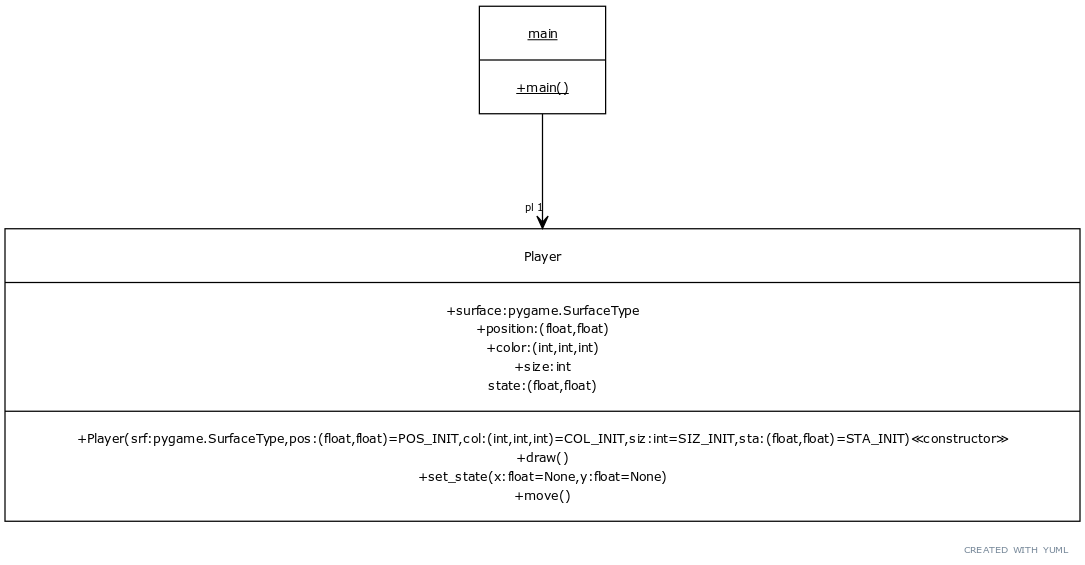
\includegraphics[scale=0.34]{./img/yuml-1}

Die erste halbwegs funktionierende Version: Ein gelber Punkt bewegt sich auf einem grauen Bildschirm

\subsection{Stand 23.11.2021}

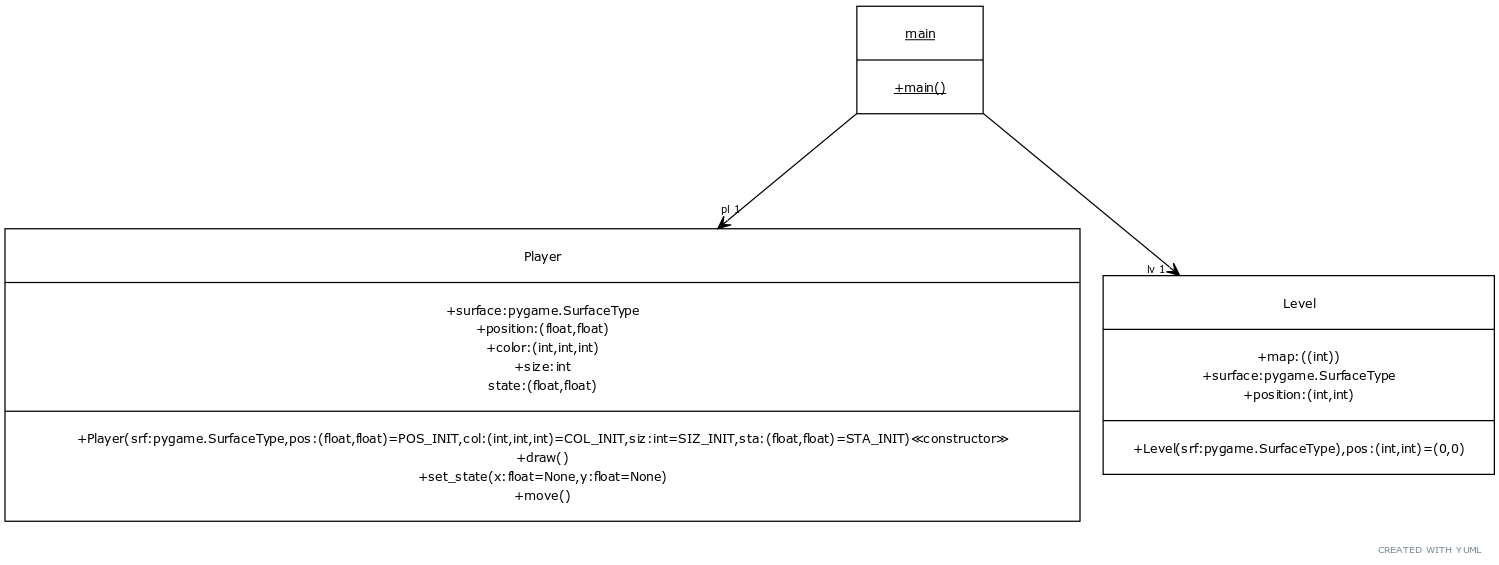
\includegraphics[scale=0.25]{./img/yuml-2}

Nun wird eine Karte auf der linken Hälfte des Fensters angezeigt.

\subsection{Stand 02.12.2021}

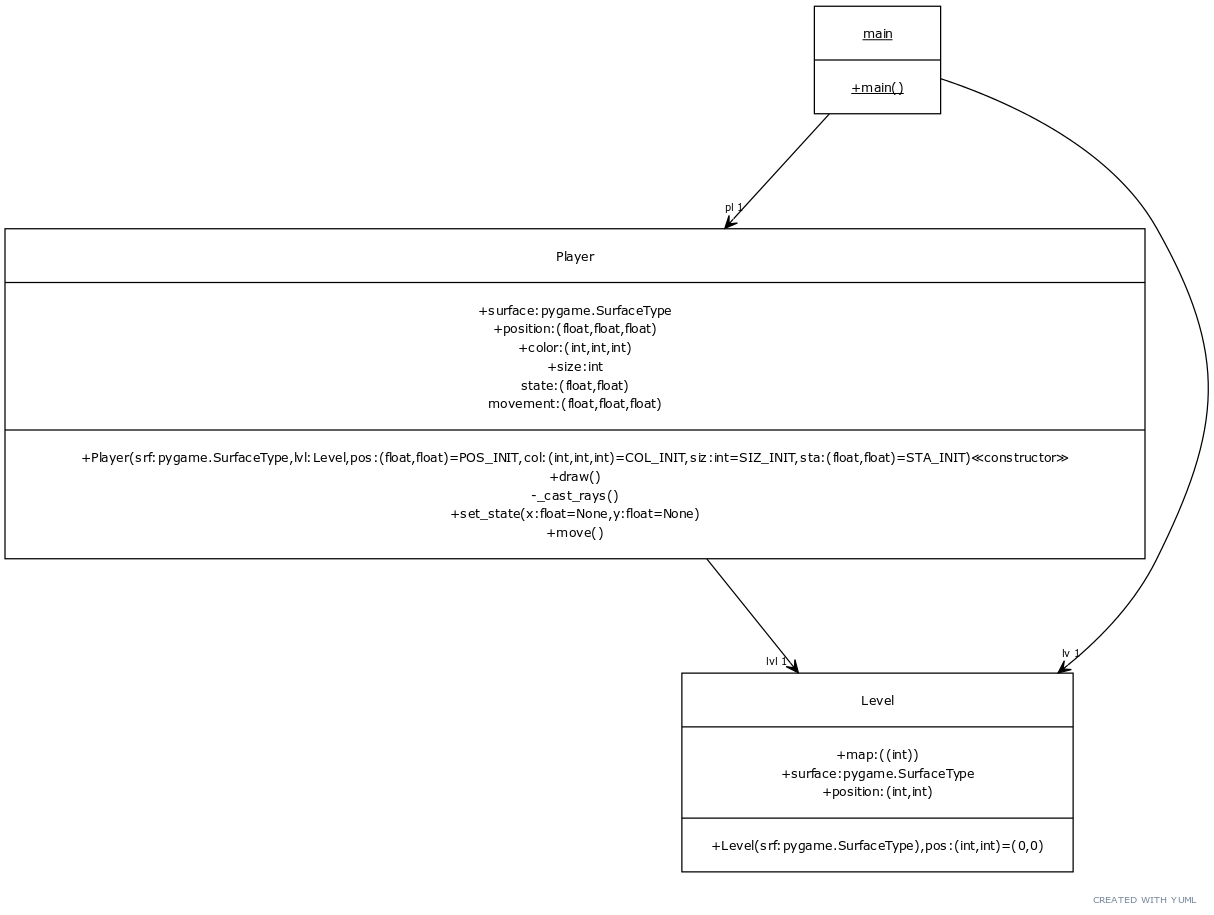
\includegraphics[scale=0.31]{./img/yuml-3}

Das Bewegungssystem wurde fast vollständig erneuert, damit sich der Spieler drehen kann und die erste Version Raycasting wird nun auf der Karte angezeigt.

\subsection{Stand 09.12.2021}

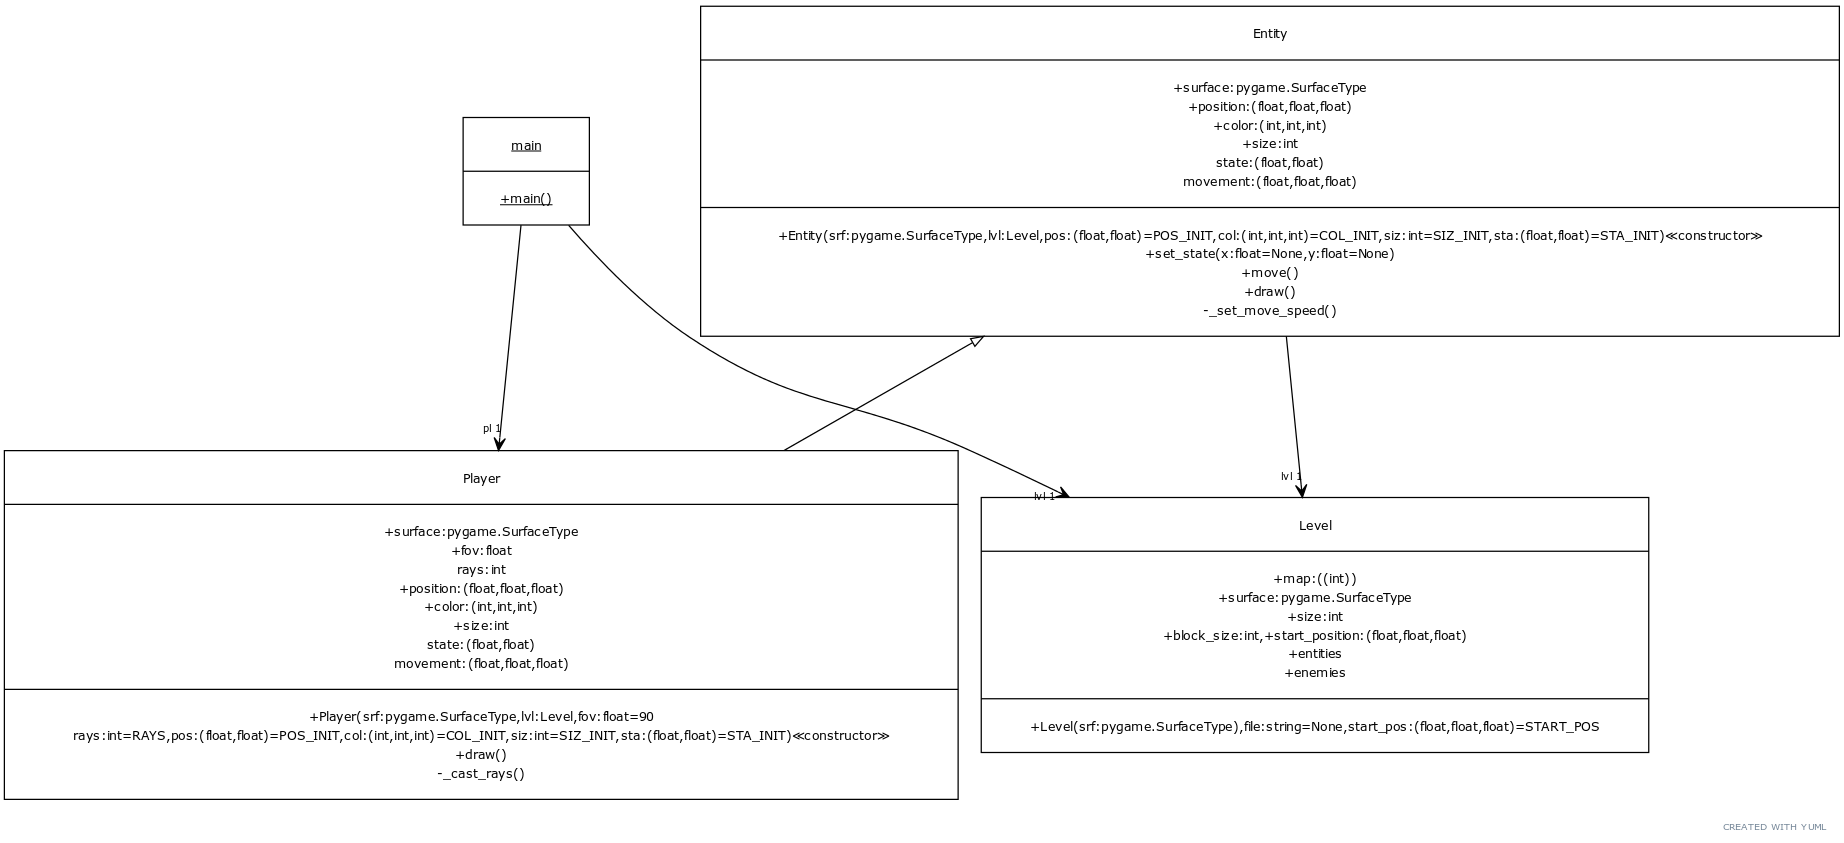
\includegraphics[scale=0.2]{./img/yuml-4}

In der rechten Hälfte des Fensters wird jetzt der First-Person Viewport angezeigt, ausserdem unterstützt das Programm jetzt Command-line Argumente.

\subsection{Stand 07.01.2022}

Dies ist die finale Version, sie entspricht dem UML-Diagramm in Abschnitt 4.

Jetzt können auch Objekte in der Karte und im Viewport angezeigt werden, zusätzlich gibt es sehr rudimentäre Kollision.

\newpage

\section{Steuerung}

\subsection{Start und Command-Line Argumente}

Gestartet wird das Spiel mit \verb|py main.py| bzw. \verb|python3 main.py|.

\begin{itemize}
	\item \verb|-h --help| zeigt die CLI Argumente und beendet das Programm.
	\item \verb|-l --level| lädt das angegebene Level oder die angegebene Level Datei.
	\item \verb|--fov| ändert den Blickwinkel (angegeben in Grad) Standartwert ist 90°.
	\item \verb|--rays| ändert die horizontale Auflösung (Anzahl der gesendeten Strahlen) Standartwert ist 90. Höhere Werte können die Leistung beeinträchtigen.
\end{itemize}

\subsection{Levelerstellung}
Level werden im JSON-Format gespeichert.
\begin{itemize}
	\item \verb|"map": [[int]]| Die Map: 1 entspricht einer Wand, 0 Leerraum. Die Map muss quadratisch sein (ansonsten crasht das Programm)
	\item \verb|"size": int| Die Größe der Map. Muss dem tatsächlichen Wert entsprechen.
	\item \verb|"start_pos": [x: int, y: int, r: int]| Die Startposition des Spielers. \verb|x| und \verb|y| sind Werte zwischen 0 und 512, sie geben die Position in Pixeln an. \verb|r| ist zwischen 0 und 360 und ist die Drehung in Grad.
	\item \verb|"entities": [], "enemies": []| Enthalten aktuell keine Werte und werden für zukünftigen Gebrauch freigehalten.
	
\end{itemize}

\subsection{Bewegung}

\subsubsection*{Translation (Laufen)}
\begin{itemize}
\item Vorwärts: `W'
\item Links: `A'
\item Rückwärts: `S'
\item Rechts: `D'
\end{itemize}

\subsubsection*{Rotation}
\begin{itemize}
\item Links: linke Pfeiltaste ($\leftarrow$)
\item Rechts: rechte Pfeiltaste ($\rightarrow$)
\end{itemize}

\subsection{UI}
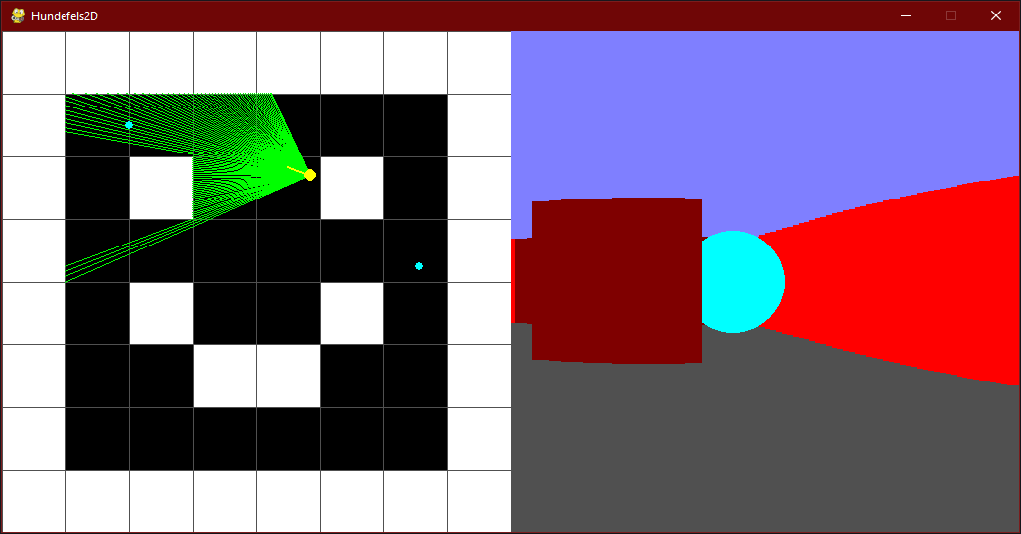
\includegraphics[scale=0.5]{./img/ui3}\\
Das Anzeigefenster ist 1024 auf 512 Pixel groß.

Die linke Hälfte enthält die Kartenansicht. Der Spieler wird mit einem gelben Punkt darestellt, Entities mit (standartmässig) blauen Punkten.

Die rechte Hälfte des Fensters ist der First-Person Viewport.

\newpage

\section{Quellen}

\begin{itemize}
	\item 3DSage: ~ ``Make Your Own Raycaster Part 1'' ~ \verb|https://youtu.be/gYRrGTC7GtA|\\ Quellcode verfügbar unter \verb|https://github.com/3DSage/OpenGL-Raycaster\_v1|
	
	Für die Raycasting-Logik (Inhalt der Funktion \verb|_cast_rays()| in \verb|player.py|)
	
	\item Pygame tutorial: \verb|https://www.pygame.org/docs/tut/MakeGames.html|
\end{itemize}


\end{document}